
\chapter{Wykorzystane narzędzia, technologie i~protokoły}

\section{LoRa}
LoRa (Long Range) to protokół komunikacji bezprzewodowej, stworzony z myślą o~urządzeniach IoT.
Przeznaczony jest do komunikacji na duże odległości i~z~niskim zużyciem energii.
Został opracowany przez Semtech w 2013 roku, stał się wtedy otwartym standardem.
LoRa wykorzystuje zastrzeżoną technologię modulacji widma rozproszonego, która umożliwia daleki zasięg, przy ograniczonym zużyciu energii.
Implementuje on warstwę fizyczną sieci~\cite{lora:about}.

Teoretyczny zasięg sieci LoRa wynosi około 15 km w terenie wiejskim i 2--5 km w terenie zurbanizowanym.
W praktyce zasięg ten jest ograniczony przez wiele czynników, takich jak:
\begin{itemize}
    \item moc nadajnika
    \item czułość odbiornika
    \item przeszkody fizyczne
    \item zakłócenia
    \item wysokość anteny
\end{itemize}
Więcej na temat wydajności sieci można przeczytać w~artykule~\cite{bib:lora-performance}.

\section{Urządzenia wykorzystywane w~projekcie}

\subsection{ESP32}
ESP32 to jednoukładowy mikrokontroler, zaprojektowany i~produkowany przez firmę Espressif Systems.
Jego najważniejsze cechy to:
\begin{itemize}
    \item energooszczędny procesor RISC o częstotliwości do 240 MHz
    \item 520 kB pamięci SRAM
    \item WiFi 802.11 b/g/n
    \item Bluetooth
    \item liczne interfejsy cyfrowe i analogowe, w~tym:
          \begin{itemize}
              \item UART
              \item I2C
              \item SPI
              \item I2S
              \item CAN
              \item ADC
              \item DAC
              \item PWM
              \item Ethernet MAC
              \item USB 2.0
          \end{itemize}
    \item \dots
          % \item 32 MB pamięci flash
\end{itemize} \cite{ESP32:datasheet}

Powstało wiele wersji tego układu, różniące się m.in. szybkością procesora, wielkością pamięci flash, ilością pinów, interfejsów cyfrowych i~analogowych, a~także możliwością pracy w trybie bezprzewodowym (WiFi) lub przewodowym (Ethernet)~\cite{ESP32:socs}.
Najczęściej układ te wykorzystywane różnych projektach IoT, zarówno jako czujniki, jak i~serwery~\cite{ESP32:datasheet}.


%  PROJECTS
W projekcie ESP32 zostało wykorzystane w dwóch płytkach TTGO T3 V1.6.1.
Jedna z płytek została wykorzystana jako przekaźnik danych pomiędzy siecią LoRa a~siecią WiFi, a druga jako cześć systemu zbierania danych z wykorzystaniem LoRa.


\subsection{Raspberry Pi Pico}

Raspberry Pi Pico to płytka z mikrokontrolerem RP2040, zaprojektowana i~produkowany przez firmę Raspberry Pi Foundation.
Charakteryzuje się ona dwurdzeniowym procesorem ARM Cortex-M0+ o~częstotliwości 133 MHz, 264 kB pamięci SRAM oraz 2 MB pamięci flash.
Płytka posiada również wiele interfejsów cyfrowych i~analogowych, w~tym:
\begin{itemize}
    \item UART
    \item I2C
    \item SPI
    \item I2S
    \item ADC
    \item DAC
    \item PWM
    \item USB 1.1
\end{itemize}~\cite{PICO:datasheet,PICO:doc}
Płytka ta jest często wykorzystywana przez hobbystów do różnych projektów IoT, a~także jako sterownik silników, czy kontroler robotów\cite{PICO:doc}.

%  PROJECTS
W projekcie dwie płytki zostały wykorzystane jako część systemu zbierania danych.
% \subsection{STM32}
% STM32 to rodzina 32 bitowych mikrokontrolerów produkowanych przez firmę STMicroelectronics. Bazują one na architekturze ARM Cortex-M, oferują wysoką wydajność i energooszczędność. Cztery główne rodzaje mikrokontrolerów STM32 to:
% \begin{itemize}
%     \item Rodzina płytek z~częścią kodu F(4/5) i H — overują największą wydajność
%     \item Rodzina płytek z~częścią kodu L — oferują największą energooszczędność
%     \item Rodzina płytek z~częścią kodu G/C/F(1/3) — do zastosowań ogólnych
%     \item Rodzina płytek z częścią kodu W(L/B/BA) — do zastosowań bezprzewodowych. [SRPAWDZIĆ]
% \end{itemize}\cite{STM32:overview}
% Głównym zastosowaniem STM32 są urządzenia wbudowane, w~tym urządzenia medyczne, roboty, samochody, a~także urządzenia IoT[NEED CITE]
% % -- PROJECTS
% \\
% W projekcie wykorzystano dwie płytki STM32WL55, które zostały wykorzystane jako część systemu zbierania danych.


\section{Języki programowania i technologie}
% \subsection{\texttt{C++} for Arduio}
% ---
\subsection{\texttt{MicroPython} for Raspberry Pi Pico}
MicroPython to lekka~i wydajna implementacja języka Python 3, która została zaprojektowana~z myślą~o urządzeniach wbudowanych.
Zawiera on okrojoną wersję biblioteki standardowej Pythona.
MicroPython jest dostępny na wiele platform,~w tym na Raspberry Pi Pico~\cite{PICO:micropython}.

\section{Protokoły komunikacyjne}

\subsection{\texttt{MQTT}}
MQTT (MQ Telemetry Transport) to lekki protokół przesyłania wiadomości, często wykorzystywany w IoT, gdzie ważna jest energooszczędność.
Oparty jest o model publish/subscribe.
Oznacza to zorganizowanie wiadomości w tematy, a klienci mogą subskrybować określone przez siebie tematy, aby otrzymywać odpowiednie wiadomości.
Zapewnia to wydają komunikację przy małym obciążeniu systemu~\cite{protocol:mqtt}.

\section{Bazy danych i pozostałe technologie}
\subsection{InfluxDB 2}
InfluxDB 2 to baza danych szeregów czasowych, stworzona przez InfluxData, Została napisana w języku Go.
Wykorzystywana jest do zbierania danych z~, między innymi, urządzeń IoT, metryk aplikacji, monitoringu infrastruktury IT~\cite{tool:influxdb}.

\subsection{Docker}
Docker to narzędzie do wirtualizacji na poziomie systemu operacyjnego.
Pozwala ono na uruchamianie aplikacji w~kontenerach, które są odizolowane od siebie i~od systemu operacyjnego.
Kontenery są lżejsze od wirtualnych maszyn, ponieważ nie muszą zawierać systemu operacyjnego, a~tylko potrzebne do działania aplikacji biblioteki i~pliki~\cite{tool:docker}.

\subsection{PlatformIO}
PlatformIO to narzędzie do tworzenia i~zarządzania projektami z~wykorzystaniem mikrokontrolerów.
Pozwala ono na tworzenie projektów w~językach C i~C++.
PlatformIO oferuje również możliwość zarządzania zależnościami projektu, zarządzania bibliotekami, a~także kompilację i~wgrywanie projektu na płytkę.
Najważniejszą cechą jest możliwość tworzenia projektów dla wielu platform i z wykorzystaniem równych narzędzi, w~tym dla ESP32 i~Raspberry Pi Pico, będąc jednocześnie niezależnym od jednego producenta~\cite{tool:pio}.

\begin{figure}[b!]
    \begin{center}
        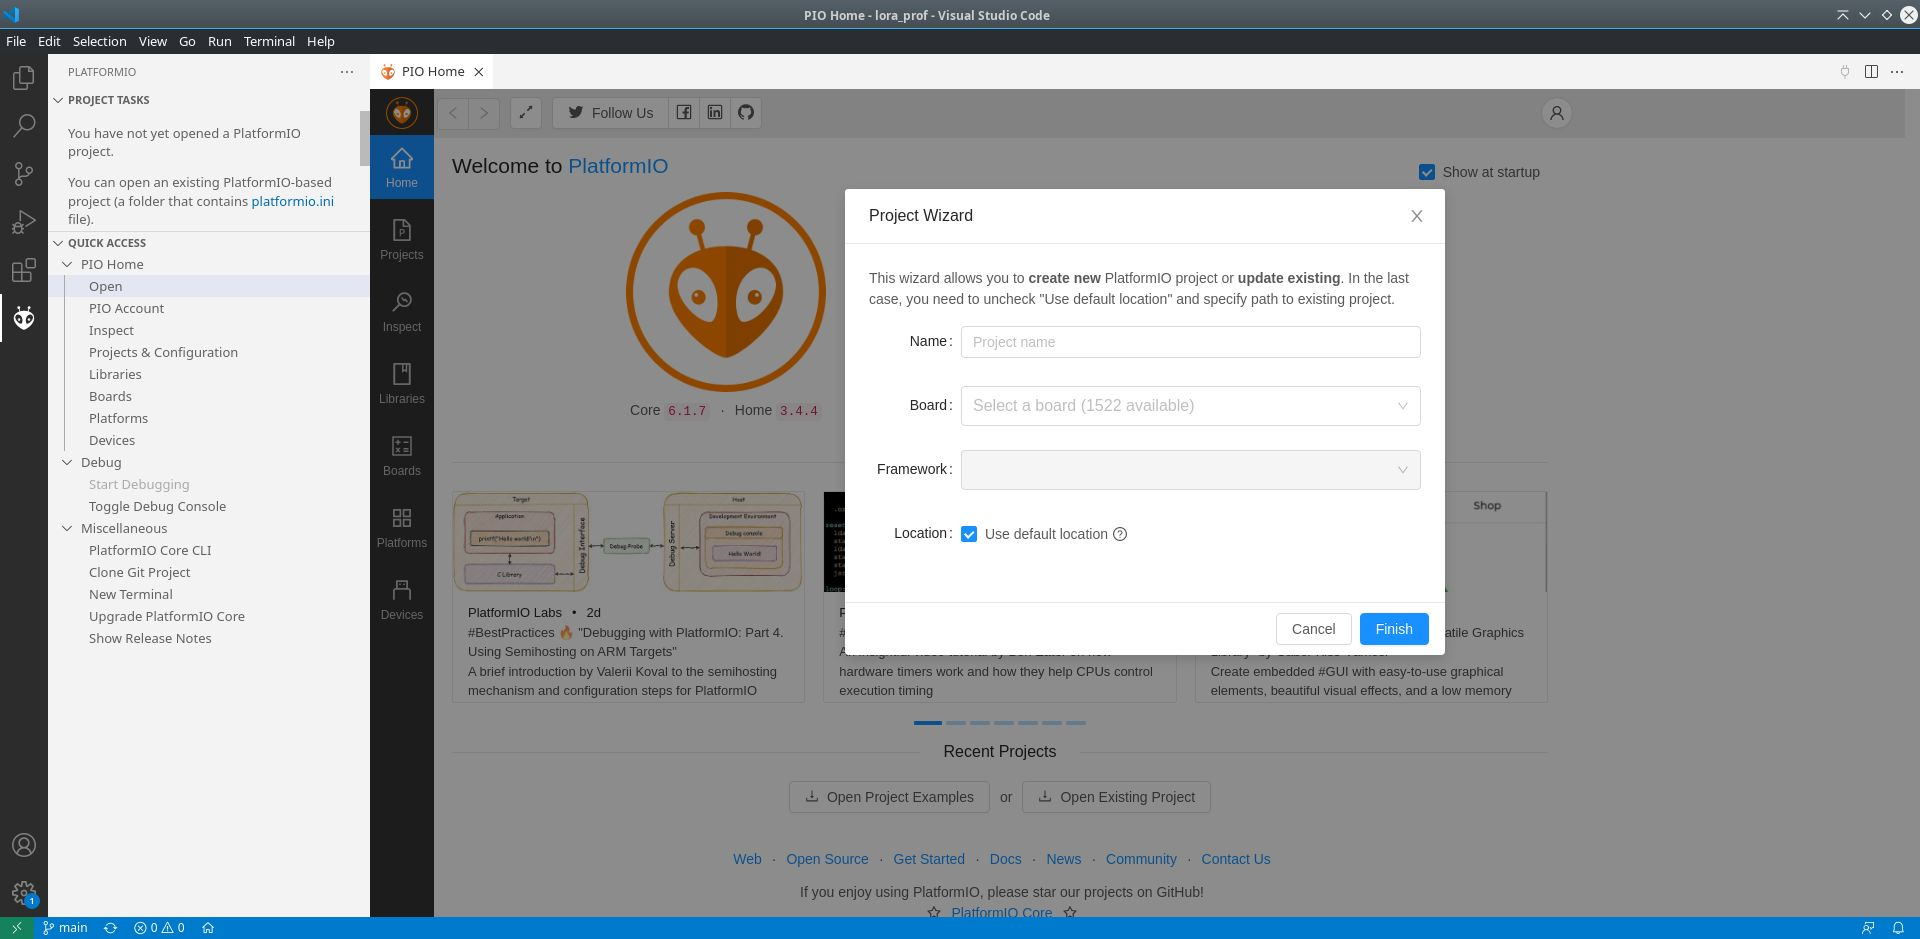
\includegraphics[width=15cm]{pic/pio.jpg}
    \end{center}
    \caption{Interfejs narzędzia PlatformIO w edytorze Visual Studio Code}\label{fig:pio}
\end{figure}
